\renewcommand\textfraction{.15}
\renewcommand\bottomfraction{.6}
\renewcommand\topfraction{.6}
\newcommand\gnuplotsource[2]{
\begin{figure}[b]
\footnotesize
\begin{multicols}{2}
\verbatiminput{#1}
\end{multicols}
\caption{#2}
\end{figure}
}

\Level 0 {Introduction to curve approximation}

You may never have thought of it, but fonts (actually, typefaces)
usually have a mathematical definition somehow. If a font is given as
a bitmap, this is typically the result from a more compact
description. Imagine the situation that you have bitmaps at 300dpi,
and you buy a 600dpi printer. It wouldn't look pretty.

There is then a need for a mathematical way of describing arbitrary
shapes. These shapes can also be three-dimensional; in fact, a~lot of
the mathematics in this chapter was developed by a car manufacturer
for modeling car body shapes.
But let us for now only look in two dimensions, which means that the
curves are lines, rather than planes.

A~mathematical formalism for curves should have these properties:
\begin{itemize}
\item The description should be clear and unambiguous.
\item It should be easy to tinker with the shapes. This is important
  for the design phase.
\item Constructing and evaluating the curves should be computationally
  cheap.
\item The curves should be well behaved: small changes in the
  definition should not lead to unexpected bulges or spikes.
\item Curves should be easily composable: if two curves describe
  adjacent pieces of the shape, they should connect smoothly.
\end{itemize}

We actually have two problems that we want to solve:
\begin{enumerate}
\item The exact curve is known, and we want to approximate it, for
  instance by something that is cheaper to compute, or
\item Only certain points are given, and we want to draw a smooth
  curve through them.
\end{enumerate}
We will tackle the second problem first.

\Level 1 {Interpolation}

\index{Interpolation}
The interpolation problem is that of, given points
$(x_1,f_1)\ldots(x_n,f_n)$, drawing a curve through them, for instance
for purposes of computing intermediate values.
Suppose that we have decided on a polynomial for the interpolating curve. With
$n$~points we need an $n-1$st degree polynomial
$p(x)=p_{n-1}x^{n-1}+\cdots+p_1x+p_0$, which takes
$n$~coefficients. We can draw up the set of equations~$p(x_i)=f_i$ and
solve that. The system
\begin{eqnarray*}
p_{n-1}x_1^{n-1}+\cdots+p_1x_1+p_0&=&f_1\\
&\ldots\\
p_{n-1}x_n^{n-1}+\cdots+p_1x_n+p_0&=&f_n
\end{eqnarray*}
can be written as $X\bar p=\bar f$, where
\[ X=\bigl(x_i^j\bigr),\quad
   \bar p=\pmatrix{p_1\cr \vdots\cr p_{n-1}},\quad
   \bar f=\pmatrix{f_1-p_0\cr \vdots\cr f_n-p_0}
   \]
Solving this system is not overly expensive, but its numerical
stability is questionable. A better way of computing the same
polynomial~$p$ is to define auxiliary polynomials~$p^{(k)}$:
\[ p^{(k)}(x) = c_k
    (x-x_1)\cdots(x-x_{k-1})\,(x-x_{k+1})\cdots(x-x_n) \]
where $c_k$ is chosen so that~$p^{(k)}(x_k)=1$.
From the fact that
$p^{(i)}(x_j)=\delta_{ij}$, it follows that
\begin{equation} p(x) = \sum_i f_ip^{(i)}(x),\qquad
    p^{(i)}(x)=\prod_{j\not=i}{x-x_j\over x_i-x_j}
    \label{eq:lagrange}\end{equation}
interpolates the points as intended. It is easy enough to prove that
polynomials are uniquely defined by these interpolation points, so we
have now computed the same polynomial in a more stable way.
A~polynomial that is based on exact interpolation of values in a
number of points is called a~`\index{Lagrange
  interpolation}\index{Interpolation!Lagrange}Lagrange interpolation'
polynomial.

Another type of interpolation is `\index{Hermite
  interpolation}\index{Interpolation!Hermite}Hermite interpolation',
where the derivatives are dictated, rather than function
values. Analogous to the above construction, we can define polynomials
\[ q^{(k)} = c_k
    (x-x_1)^2\cdots(x-x_{k-1})^2\cdot (x-x_k)\cdot
    (x-x_{k+1})^2\cdots(x-x_n)^2 \]
where $c_k$ is chosen so that $q^{(k)'}(x_k)=1$.

\Level 1 {Approximation}

\index{Approximation, of curves}
The above notion of interpolation is sometimes applied to known
curves. For instance, by finding an interpolating polynomial we may
aim to find a cheaper way of computing values on
the curve. This raises the question how well the interpolation curve
approximates the original curve.

In classical approximation theory there is usually a family of
functions~$\{f_n\}$, typically polynomials of increasing degree, such
that $\|f_n-f\|\rightarrow0$, typically on a closed interval~$I$. The
Weierstrass approximation theorem tells us that every continuous
function on a closed bounded interval can be approximated by
polynomials.

\begin{figure}[t]
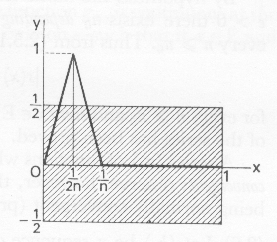
\includegraphics{hat-function}
\caption{A family of functions that converges pointwise but not
  uniformly.}
\label{fig:hatfunc}
\end{figure}
Note that this is uniform convergence:
\[ \forall_\epsilon\exists_N\forall_{x\in I,n\geq N}:
    \left|f_n(x)-f(x)\right|\leq\epsilon.
\]
This is a stronger statement than pointwise convergence:
\[ \forall_{x\in I,\epsilon}\exists_N\forall_{n\geq N}:
    \left|f_n(x)-f(x)\right|\leq\epsilon.
\]
It is easy to find families of functions~$f_n$ that convergence in the
pointwise sense, but not uniformly; see figure~\ref{fig:hatfunc}.

The spline curves that we will study later in this chapter are a
special case of Bernstein polymials: the $n$-th Bernstein polynomials
for a function~$f$ is
\[ B_n(f)(t) = \sum_{p=0}^n \bigl({n\atop p}\bigr)
    f\bigl({p\over n}\bigr)(1-t)^{n-p}t^p. 
\]
If $f$ is continuous on~$[0,1]$, this sequence converges uniformly
to~$f$. It is worth remarking that these polynomials do not require
computation of derivatives.

While the ideas behind Lagrange and Hermite interpolation will find
applicability later in this story, the idea of interpolating with a
single, high degree, polynomial may not be a good one from a point of
uniform convergence. The error can
be unacceptably large, as can be seen in figure~\ref{fig:runge}, where
the dashed line is an interpolation on equispaced points. In this case
there is in fact not even pointwise convergence.
\begin{figure}[t]
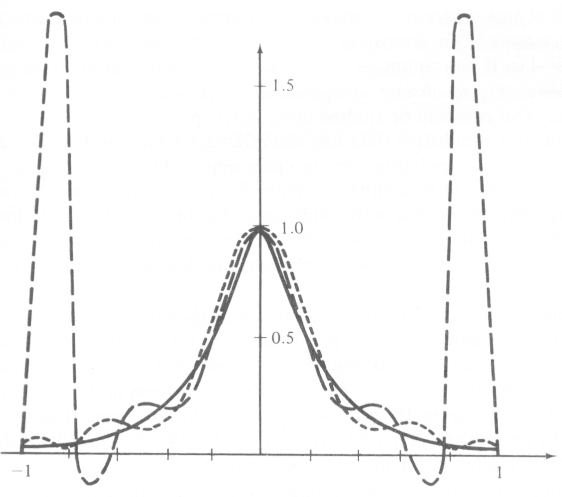
\includegraphics[scale=.7]{runge}
\caption{The Runge effect of interpolating with a high degree polynomial}
\label{fig:runge}
\end{figure}
There are a few ways out of that, such as
better choice of interpolation points or of basis functions.
In figure~\ref{fig:runge} the dotted line uses Tchebyshev
interpolation points which is seen to remedy the problem to a large
extent.

However, the approach we will use here is that of piecewise
approximations with relatively low degree polynomials. This simplifies
certain aspects, but we need to take care to piece together such
curves smoothly.  For instance, with Lagrange interpolation the
direction of the curve at the end points can not be specified.

\Level 1 {Computation with interpolation curves}

While we will mostly investigate theoretical properties of
interpolation curves, the practical matter of how efficient it is to
work with them, also deserves attention. In \eqref{eq:lagrange} there
are $n$~terms involving $n$~multiplications and additions each, making
for an $O(n^2)$~cost. This can be considerably reduced by rewriting
the formula as
\[ p(x) = \prod_i(x-t_i)\cdot\sum_i{y_i\over x-t_i},
    \qquad y_i=f_i/\prod_{j\not=i}(x_i-x_j),
\]
which takes $n$~additions, multiplications, and additions if the
$y_i$~quantities are precomputed. We will now see a formulation that
dispenses with the divisions, and that will also be simpler if
derivatives need to be computed.

\newcommand\kdd[1]{\kddl{1}{#1}}
\newcommand\kddl[2]{[\tau_{#1},\ldots,\tau_{#2}]}

The $k$-th
`\index{divided difference}divided difference' of a function~$g$ in
the points $\tau_1\ldots\tau_{k+1}$, notation $\kdd{k+1}g$, is the
leading coefficient of the $k$-th order\footnote{It is convenient to
  talk about polymomials of a certain order rather than degree:
  a~polynomial of order~$k$ has a degree no more than~$k$. We denote
  this set with~$\prod_{<k+1}$. One advantage of this set is that it
  is closed under summing.}  polynomial~$p_{k+1}$ that agrees with~$g$
in the points~$\tau_1\ldots\tau_{k+1}$.

The simplest examples of divided differences are:
\begin{itemize}
\item The zeroeth divided difference of a function is the leading
  coefficient of a zeroth order polynomial $p(x)=c$ that agrees with
  that function in one point: $g(\tau_1)=g_1$. Clearly $[\tau_1]g=g_1$.
\item The first divided difference is the leading coefficient of a
  linear function that agrees in two points:
\[ [\tau_1,\tau_2]g={g(\tau_2)-g(\tau_1)\over \tau_2-\tau_1}
    ={[\tau_2]g-[\tau_1]g\over \tau_2-\tau_1}
\]
This equation may suggest to the reader a relation for higher divided
differences. We shall see in lemma~\ref{lemma:divdiff-construct} that
this indeed holds.
\end{itemize}

We now prove some facts about divided differences.
\begin{lemma}\label{lemma:pk-diff}
Let $p_{k+1}\in\prod_{<k+1}$ agree with~$g$ in
$\tau_1\ldots\tau_{k+1}$, and $p_k\in\prod_{<k}$ with~$g$ in
$\tau_1\ldots\tau_k$, then
\begin{equation}
    p_{k+1}(x)-p_k(x)=\kdd{k+1}g\prod_{i=1}^k(x-\tau_i).
    \label{eq:pk-diff}
\end{equation}
\end{lemma}
Proof. Since $p_k$ is of a lower order, we immediately have
\[ p_{k+1}-p_k=\kdd{k+1}gx^k+cx^{k-1}+\cdots.\]
Observing that $p_{k+1}-p_k$ is zero in~$t_i$ for~$i\leq\nobreak k$,
it follows that
\[ p_{k+1}-p_k=C\prod_{i=1}^k(x-\tau_i). \]
From this we get that $C=\kdd{k+1}g$.\endproof

If we repeat this lemma we find that 
\begin{equation}
    p_{k+1}(x)=\sum_{m=1}^{k+1}\kdd{m}g\prod_{i=1}^{m-1}(x-\tau_i),
    \label{eq:p-sum-diffs}
\end{equation}
which we can evaluate as 
\[
\begin{array}{rcl}
 p_{k+1}(x) &=&
 \kdd{k+1}g\prod^k(x-\tau_i)+\kdd{k}g\prod^{k-1}(x-\tau_i)\\
    &=&\kdd{k+1}g(x-\tau_k)\bigl(c_k
                +\kdd{k}g(x-\tau_{k-1})\bigl(c_{k-1}+\cdots
\end{array}
\]
where $c_k=\kdd{k}g/\kdd{k+1}g$. This is a very efficient evaluation
by Horner's rule. 

The remaining question is how to construct the
divided differences. We approach this recursively.
\begin{lemma}\label{lemma:divdiff-construct}
Divided differences can be constructed by, eh, dividing differences
\begin{equation}
    \kdd{n+1}g=\left(\kdd{n}g-\kddl{2}{n+1}g\right)/(\tau_1-\tau_{n+1}).
    \label{eq:div-diff}
\end{equation}
\end{lemma}
Proof. Let three polynomials be given:
\begin{itemize}
\item $p^{(1)}_n\in\prod_{<n}$ agrees with~$g$ on
  $\tau_1\ldots\tau_n$;
\item $p^{(2)}_n\in\prod_{<n}$ agrees with~$g$ on
  $\tau_2\ldots\tau_{n+1}$;
\item $p_{n-1}\in\prod_{<n-1}$ agrees with~$g$ on
  $\tau_2\ldots\tau_n$.
\end{itemize}
Then by lemma~\ref{lemma:pk-diff}
\[ \begin{array}{rcl}
  p^{(1)}_n-p_{n-1}&=&\kdd{n}g\prod_{j=2}^n(x-\tau_j)\\
  p^{(2)}_n-p_{n-1}&=&\kddl{2}{n+1}g\prod_{j=2}^n(x-\tau_j)
\end{array} \]
Now let $p_{n+1}$ be the polynomial that agrees with~$g$ on
$\tau_1\ldots\tau_{n+1}$, then
\[ \begin{array}{rcl}
  p_{n+1}-p^{(1)}&=&\kdd{n+1}g\prod_{j=1}^n(x-\tau_j)\\
  p_{n+1}-p^{(2)}&=&\kdd{n+1}g\prod_{j=2}^{n+1}(x-\tau_j)
\end{array} \]
Subtracting both pairs of equations, we find two expressions for
$p^{(1)}_n-p^{(2)}_n$:
\[ \left(\kdd{n}g-\kddl{2}{n+1}g\right)\prod_{j=2}^n(x-\tau_j)
  = \kdd{n+1}g\left(\prod_{j=2}^{n+1}-\prod_{j=1}^n\right)
        (x-\tau_j)
\] 
Filling in $\tau_2\ldots\tau_n$ in this equation, we find zero for
both sides. Using~$x=\nobreak\tau_1$ we find
\[ \left(\kdd{n}g-\kddl{2}{n+1}g\right)\prod_{j=2}^n(\tau_1-\tau_j)
  = \kdd{n+1}g\prod_{j=2}^{n+1}(\tau_1-\tau_j)
\]
from which the lemma follows.\endproof

From this lemma, we see easily that $\kdd{n}g$ can be computed in
approximately $n^2/2$ additions and divisions.

\Level 0 {Parametric curves}

So far we have been looking at approximation by a function of a single
value. That is, we have $y$ as a function of~$x$. This rules out many
curves, such as circles. We could try expressing $x$ as a function
of~$y$, or more generally rotating them, but that is a big hassle, and
it would still rule out some curves.

Another approach is to let the curve be defined implicitly by
$f(x,y,z)=0$. This suffers from several problems. We could get too
many solutions, for instance as in $x^2+y^2-1=0$, requiring
constraints. Tracking a path is possible in theory, but is not trivial
in practice. Finally, many shapes are defined piecewise, and joining
shapes in a smooth way is also tricky.

Rather than considering a curve in the plane as a function, it is more
productive to describe the shape of the curve, as some imaginary point
moves over the curve. That is, we have a description of the points on
the curve as
\[ P=P(t) = \pmatrix{x(t)\cr y(t)}.\]
(Feel free to think of $t$ as time.)

A simple example of how this works is to consider two points $P_1$
and~$P_2$, and the curve $P=tP_2+(1-t)P_1$. Then for $t=0$,
$P(0)=P_1$, for $t=1$, $P(1)=P_2$, and for intermediate values
of~$t$ we get some point between $P_1$ and~$P_2$.

That this solves our problems with multiple solutions that were
present in both function and implicit approaches is clear if we look
at the example~$P(t)=(\cos 2\pi t,\sin 2\pi t)$, which traces out a
circle as $t$ goes from $0$ to~$1$.

While a description in terms of piecewise linear functions would be
very simple, it is not smooth.  Using the various ideas sketched
above, we will now concentrate on curves that are piecewise parametric
cubic splines. Cubics have the following property that they are the
lowest degree that allows specification of location and direction in
the end points. Higher degree functions would allow for instance the
specification of higher derivatives, but unless great care is taken,
they would introduce unwanted `wiggles' in the curves.

Using piecewise cubic parametric curves then is a good mean between
ease of use and power of approximation.

\Level 1 {Parametrized basis functions}

To begin with we will concentrate on a single curve~$Q(t)$ where
$t=0\ldots1$. We often write this as $Q(t)=C\cdot T$ where
the coefficient matrix
\[ C=\pmatrix{c_{11}&c_{12}&c_{13}&c_{14}\cr
    c_{21}&c_{22}&c_{23}&c_{24}\cr c_{31}&c_{32}&c_{33}&c_{34}\cr}
    ,\qquad 
    T=\pmatrix{1\cr t\cr t^2\cr t^3}
\]
The direction of the curve is then given by
\[ {dQ(t)\over dt}=C\cdot {dT\over dt}=
    C\cdot\pmatrix{0\cr 1\cr 2t\cr 3t^2}
\]
We see that the $C$~matrix can be derived if we know a total of four
locations or directions of the curve. For instance, if $P_1=Q(0)$,
$R_1=Q'(0)$, $P_2=Q(1)$, and~$R_2=\nobreak Q'(1)$ are given, then
\[ C\cdot \pmatrix{1&0&1&0\cr 0&1&1&1\cr 0&0&1&2\cr 0&0&1&3\cr}
    =[P_1,R_1,P_2,R_2],
\]
from which $C$~follows.

Now, often we have a set of basis polynomials given, and we want to
take combinations of them to satisfy the constraints. That can be
done by splitting $C=GM$, where $M$~describes the basis polynomials,
and $G$~is the `\index{geometry matrix}geometry matrix'. We get the equation
\begin{equation}
  Q(t) = G\cdot M\cdot T = 
    \pmatrix{g_{11}&g_{12}&g_{13}&g_{14}\cr
        g_{21}&g_{22}&g_{23}&g_{24}\cr g_{31}&g_{32}&g_{33}&g_{34}\cr}
    \cdot \pmatrix{m_{11}&\ldots&m_{14}\cr \vdots&&\vdots\cr
        m_{41}&\ldots&m_{44}\cr}
    \cdot T
\label{eq:geom}
\end{equation}
If we introduce new basis polynomials $\pi_i(t)=M_{i*}\cdot T$, then we
see that $Q_x=G_{11}\pi_1+G_{12}\pi_2+G_{13}\pi_3+G_{14}\pi_4$,
$Q_y=G_{21}\pi_1+\cdots$, et cetera.

\Level 1 {Hermite basis functions}

In \eqref{eq:geom} the matrix~$M$ describes the basis functions, so it
is fixed for a certain class of curves: we will have one set of basis
functions for Lagrange type curves, one for Hermite curves, et
cetera. However, we have not yet seen a way to compute the matrix~$M$.

The geometry matrix~$G$ is used to derive a specific curve in the
class described by~$M$: each choice of~$G$ corresponds to one
curve. The columns of~$G$ will be points or direction vectors that
somehow describe the intended curve.

Let us now consider Hermite curves. Here we want $G$~to be the matrix
of geometric constraints, $[P_1,R_1,P_2,R_2]$~in the above
example. Recall that these constraints, using the locations of the end
points and the derivatives of the curve there, give us indeed an example of
Hermite interpolation.

We write out the equations. From $Q=G\cdot M\cdot T$ we get
\[ Q(t)= G_H\cdot M_H\cdot T(t),\qquad
   Q'(t)= G_H\cdot M_H\cdot T'(t). \]
Applying both these formulas to $t=0$ and $t=1$, we get
\[ Q_H\equiv[Q(0),Q'(0),Q(1),Q'(1)] = G_H\cdot M_H\cdot T_H \]
where
\[ T_H=[T(0),T'(0),T(1),T'(1) ]
     =\pmatrix{1&0&1&0\cr 0&1&1&1\cr 0&0&1&2\cr 0&0&1&3\cr}
\]
But this $Q_H$ is the matrix that we had stipulated as the matrix of
geometry constraints, in other words: $G_H=Q_H$. It now follows that
\[ M_H=T_H^{-1}
    =\pmatrix{1&0&-3&2\cr 0&1&-2&1\cr 0&0&3&-2\cr 0&0&-1&1}.
\]
Writing this out, we find the cubic Hermite polynomials
\[ P_1(t)=2t^3-3t^2+1,\quad P_2(t)=t^3-2t^2+t,\quad
    P_3(t)=-2t^3+3t^2,\quad P_1(t)=t^3-t^2
\]
\begin{figure}[t]
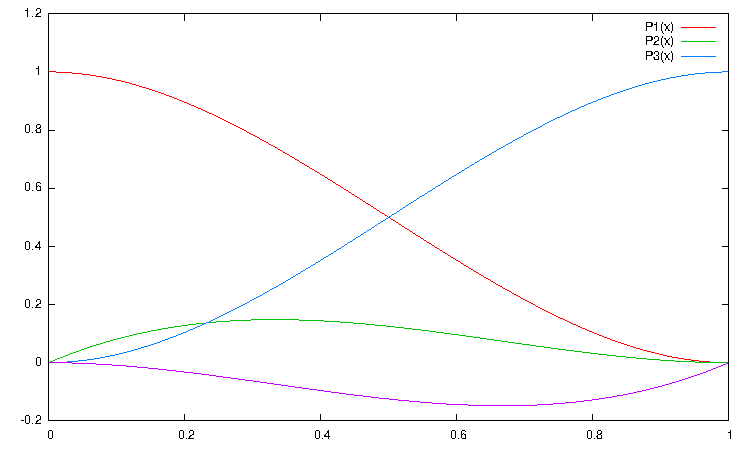
\includegraphics[scale=.7]{hermite}
\caption{Hermite polynomials}
\label{fig:hermite}
\end{figure}
\gnuplotsource{hermite.gp}{The \gnuplot\ source for figure~\ref{fig:hermite}}
illustrated in figure~\ref{fig:hermite}, and we get $Q(t)=G\cdot B_H$ where
$B_H=M\cdot T$ is the matrix of `Hermite blending functions'.

With this formula, we can take a set of geometric constraints, in this
case the two endpoints and the directions there, and derive the
formula for the Hermite curve that satisfies these constraints.
As an example, figure~\ref{fig:herminp} is the curve $.3P_1-2P_2+P_3-2P4$,
\begin{figure}[t]
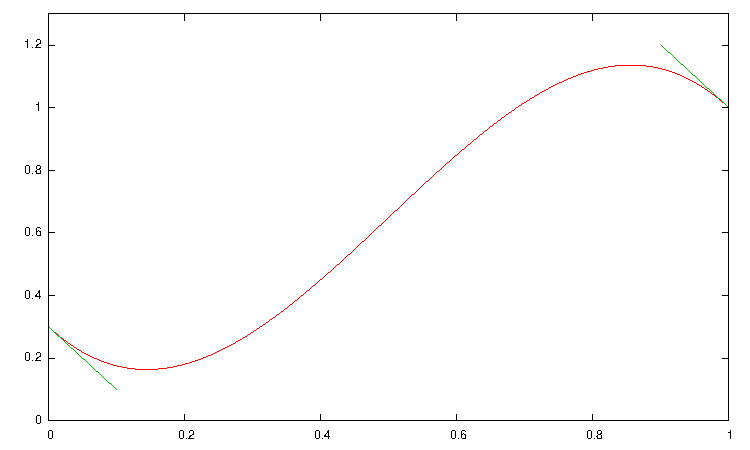
\includegraphics[scale=.7]{herminp}
\caption{An example of Hermite interpolation}
\label{fig:herminp}
\end{figure}
\gnuplotsource{herminp.gp}{The source for figure~\ref{fig:herminp}}
that is, the curve through $(0,.3)$ and~$(1,1)$, with slope~$-2$ in
both~$x=0,1$.

We make the transition to parametric curves by expressing both
components as Hermite curves. For instance, figure~\ref{fig:hermpara}
\begin{figure}[t]
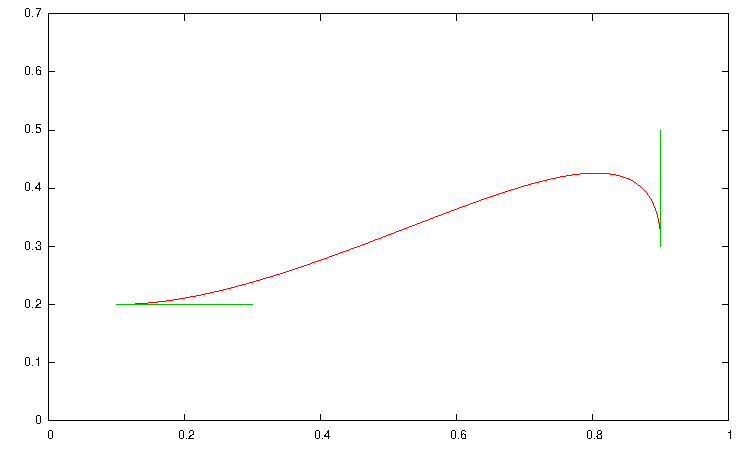
\includegraphics[scale=.7]{hermpara}
\caption{A Hermite interpolation curve}
\label{fig:hermpara}
\end{figure}
\gnuplotsource{hermpara.gp}{The source of figure~\ref{fig:hermpara}}
shows the curve
\[ Q_x(t) = .1*P_1(t)+P_2(t)+.9*P_3(t),\quad
     Q_y(t) = .2*P_1(t)+.3*P_3(t)-P_4(t)
\]
that is
\[ Q = \left({.1\atop .2}\right)P_1+\left({1\atop 0}\right)P_2
    +\left({.9\atop .3}\right)P_3+\left({0\atop -1}\right)P_4.
\]

There is one aspect of these Hermite curves worth remarking on. In
figure~\ref{fig:hermpara2} we have replaced the direction vector
$\left({1\atop 0}\right)$ in~$(0,0)$ by~$\left({x\atop 0}\right)$,
where $x=1,1.5,2,2.5$,
\begin{figure}[t]
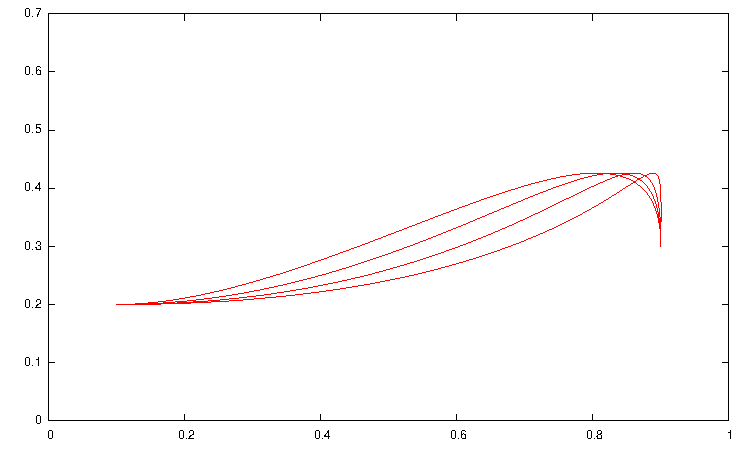
\includegraphics[scale=.7]{hermpara2}
\caption{The same curve, tinkering with the direction vector}
\label{fig:hermpara2}
\end{figure}
\gnuplotsource{hermpara2.gp}{The source for figure~\ref{fig:hermpara2}}
which all have the same direction, but a different magnitude. Clearly there
is a visual effect.

\Level 1 {Splines}

We will now take a close look at Bernshtein polynomials of degree~3:
\begin{equation} z(t)=(1-t)^3z_1+3(1-t)^2tz_2+3(1-t)t^2z_3+t^3z_4,
    \label{eq:bernshtein}\end{equation} also known as Bezier curves or
Bezier cubics after Pierre Bezier, an engineer at
Renault\footnote{Pierre B\'ezier was born September 1, 1910 and died
November 25, 1999 at the age of 89. In 1985 he was recognized by ACM
SIGGRAPH with a `Steven A. Coons' award for his lifetime contribution
to computer graphics and interactive techniques.}.

There are a couple of ways of looking at these polynomials. Consider
the function $z(t)$ to be the sum of four basis functions, $(1-t)^3$,
$(1-t)^2t$, $(1-t)t^2$, and~$t^3$, each multiplied by a factor
deriving from a control point.
From the formulas, and from a picture (figure~\ref{fig:bernsh})
\begin{figure}[t]
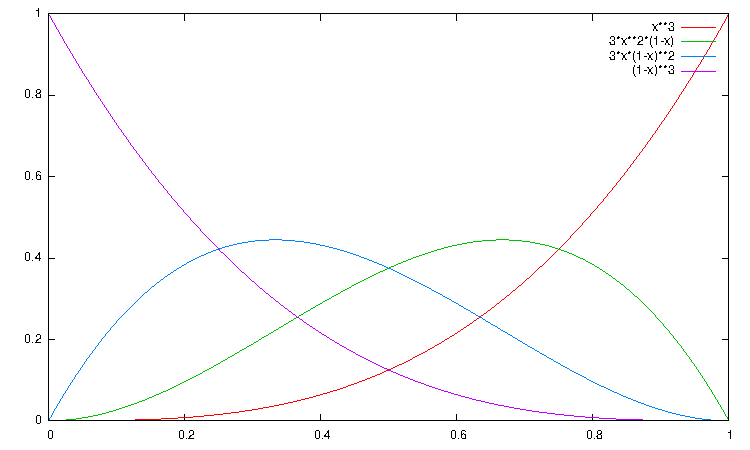
\includegraphics[scale=.7]{bernshtein}
\caption{Bernshtein polynomials}
\label{fig:bernsh}
\end{figure}
we see that the first term $p_1(t)=(1-t)^3$ is the only one with
$p(0)\not=0$. Likewise, $p_4$~is the only one with $p(1)\not=0$. That
means $z(0)=z_1$ and~$z(1)=\nobreak z_4$. Furthermore, the second term
is  (after the first term) the only remaining one with $p'(0)\not=0$,
so by choosing~$z_2$ we can change~$z'(0)$ without changing $z(0)$
or~$z(1)$. Likewise $z_3$ for~$z'(1)$.

Bezier curves can be derived from cubic Hermite splines by replacing
the direction vectors~$R_1,R_2$ by control points~$P_1',P_2'$, so that
$R_1=3(P_1'-P1)$ and $R_2=3(P_2-P_2')$. For the Bezier geometry vector
we then have
\[ G_B=[P_1,P_1',P_2',P_2] \]
and the relation with the Hermite geometry vector
\[
 G_H=[P_1,R_1,P_2,R_2]
    = [P_1,P_1',P_2',P_2] M_{BH} = G_B\cdot M_{BH}
\]
where
\begin{equation}
     M_{BH}=\pmatrix{1&-3&0&0\cr 0&3&0&0\cr 0&0&0&-3\cr 0&0&1&3\cr}
\label{eq:MBH}
\end{equation}
Defining
\begin{equation}
 M_B=M_{BH}\cdot M_H=
   \pmatrix{1&-3&3&-1\cr 0&3&-6&3\cr 0&0&3&-3\cr 0&0&0&1\cr}
\label{eq:MB}
\end{equation}
we now get for Bezier curves
\[ Q(t)=G_H\cdot M_H\cdot T(t)=G_B\cdot M_{BH}\cdot M_H\cdot T(t)
    =G_B\cdot M_B\cdot T(t)
\]
We can also write that as $Q_x(t)=g_{11}B_1(t)+g_{12}B_2(t)+\cdots$
where
\[ \begin{array}{rll}
B_1(t) &= 1-3t+3t^2 -t^3&=(1-t)^3\\
B_2(t) &= 3t-6t^2+3t^3&=3t(1-t)^2\\
B_3(t) &= 3t^2-3t^3&=3t^2(1-t)\\
B_4(t) &=          &=t^3
\end{array}
\]
which are the Bernstein polynomials we started this section with.

The sum of these polynomials (this is equivalent to setting the
$z_i$~coefficients to one in \eqref{eq:bernshtein}) is
$z(t)=(t+(1-t)))^3\equiv1$. Also, the polynomials are positive
on~$[0,1]$, so the components~$Q_x,Q_y,Q_z$ are weighted averages of
the polynomials. This means that the curve, consisting of weighted
sums of the control points, is contained in the convex hull of the
control points.
\begin{comment}
\begin{594exercise}
Fill in the missing details of this proof.
\end{594exercise}
\end{comment}

\begin{594exercise}
One could also define quadratic Bezier curves. These have only a
single control point, and the curve is such that in both the endpoints
it is aimed at the control point.\\
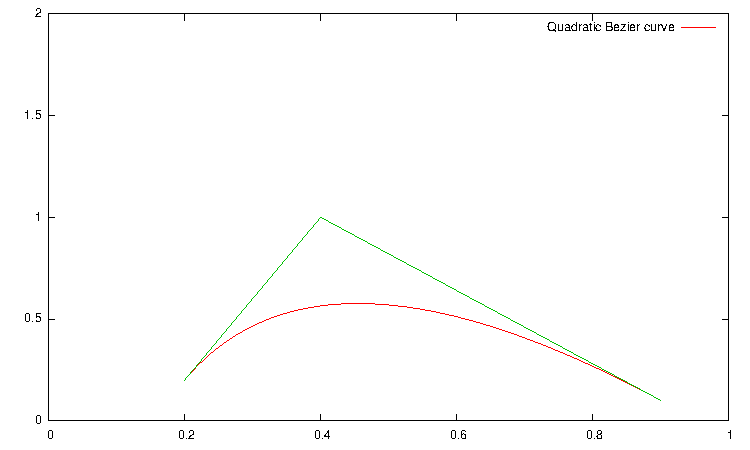
\includegraphics{bquad}\\
Derive the basis functions and geometry matrix for this case.
Make a \gnuplot\ figure of a single quadratic Bezier curve, and of two
curves joined smoothly. 

Hint: you can follow the construction of the cubic splines in the
lecture notes. The only
problem is defining the control point. First draw up the Hermite geometry matrix
based on end points $q_0$ and~$q_1$, and the derivative $q_0'$ in the
first end point. Derive from them the derivative~$q_1'$ in the other
end point. The control point then lies on the intersection of two
lines. Solving this looks like a single equation in two unknowns, but
it can be solved: write it as a matrix-vector equation that is
satisfied no matter the choice of the geometry matrix.
\end{594exercise}
\begin{answer}
Define $G_H=[q_0,q'_0,q_1]$. That gives
\[ T_H=\pmatrix{1&0&1\cr 0&1&1\cr 0&0&1},\qquad M_H=T_H\inv
    =\pmatrix{1&0&-1\cr 0&1&-1\cr 0&0&1}.
\]
The derivative in the other end point is
\[ q_1'=Q_H'(1)=G_HM_H\pmatrix{0\cr 1\cr 2}=G_H\pmatrix{-2\cr -1\cr 2}
    =2q_1-2q_0-q_0'. \]
The control point satisfies
\[ q_2=\cases{q'_0u+q_0\cr q'_1v+q_1}. \]
Substituting $q'_1$, we get
\[ Q_H\left[ \pmatrix{1\cr 0\cr-1}+\pmatrix{0&2\cr 1&1\cr 0&-2}
                \pmatrix{u\cr v}\right] = 0 \]
which is satisfied for $u=1/2$, $v=-1/2$. This gives for the Bezier
geometry matrix
\[ G_B=[q_0,q_2,q_1]=G_H\pmatrix{1&1&0\cr 0&1/2&0\cr 0&0&1},\qquad
    G_H=G_B\pmatrix{1&-2&0\cr 0&2&0\cr 0&0&1}
\]
and for the generating equation
\[ Q=G_HM_HT=G_B\pmatrix{1&-2&0\cr 0&2&0\cr 0&0&1}
    \pmatrix{1&0&-1\cr 0&1&-1\cr 0&0&1}T
    =G_B\pmatrix{1&-2&1\cr 0&2&-2\cr 0&0&1}
\]
\end{answer}

\Level 1 {Calculation of Bezier curves}
\label{sec:bezier-calc}

Suppose we have a Bezier curve defined by four control points, and we
want to draw points on the curve, meaning that we have to evaluate the
function~$Q(t)$ for a number of values of~$t$. The relation $Q(t)=G\cdot
M\cdot T(t)$ allows us to do this calculation in
\begin{itemize}
\item 2 multiplications to form the terms $t^2$ and~$t^3$ in~$T$;
\item 16 multiplications and 12 additions forming~$M\cdot T$;
\item 12 multiplications and 9 additions forming $G\cdot(M\cdot T)$.
\end{itemize}
An obvious improvement is to store $\tilde M=G\cdot M$, which brings
the cost down to two multiplications for~$T$ and 
\begin{itemize}
\item 12 multiplications and 9 additions for forming $\tilde M\cdot
  T$.
\end{itemize}
A similar count is arrived at by looking at divided
differences. Additionally, this way of computing is more stable.

From the formula $Q(t)=G\cdot M\cdot T(t)$ we get for each component
\[ q_i(t) = \sum_jG_{ij}(MT)_j = \sum_{j,k}G_{ij}M_{jk}t^{k-1}. \]
Looking at only one component for simplicity, we find, for instance
\[ x(t) = \sum_kc_kt^{k-1}\qquad c_k=\sum_jG_{1j}M_{jk}. \]
We recall \eqref{eq:MB}:
\[  M_B=\pmatrix{1&-3&3&-1\cr 0&3&-6&3\cr 0&0&3&-3\cr 0&0&0&1\cr}
\]
and writing $g_j\equiv G_{1j}$ we find
\[ c_1=g_1,\quad c_2=3(g_2-g_1),\quad
    c_3=3(g_3-2g_2+g_1),\quad c_4=g_4-3g_3+3g_2-g_1. \]
In this we recognize divided differences of~$g$:
\[ \begin{array}{lcl}\relax [2,1]g&=&g_2-g_1,\\
 \relax [3,2,1]g&=&[3,2]g-[2,1]g=(g_3-g_2)-(g_2-g_1)\\
         &=&g_3-2g_2+g_1\\
 \relax [4,3,2,1]&=&[4,3,2]g-[3,2,1]g=(g_4-2g_3+g_2)-(g_3-2g_2+g_1)\\
         &=&g_4-3g_3+3g_2-g_1
    \end{array}
\]
using lemma~\ref{lemma:divdiff-construct}.

\Level 0 {Practical use}

\Level 1 {Piecewise curves}

As we indicated earlier, complicated shapes can be approximated by
piecewise cubics. Figure~\ref{fig:herm2} shows two Hermite curves
joined together. The curve is continuous and the directions at the
join are proportional. This is called `\index{geometric
  continuity}geometric continuity', and is denoted~$G^1$.
\begin{figure}[t]
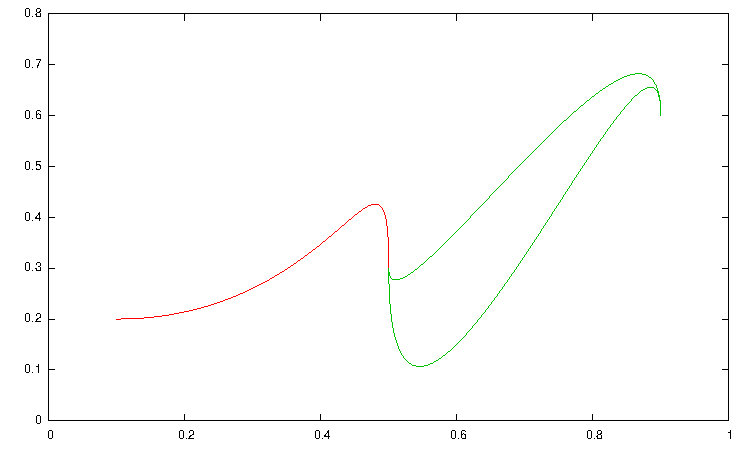
\includegraphics[scale=.7]{herm2}
\caption{Two Hermite curves, joined together smoothly in $(.5,.3)$}
\label{fig:herm2}
\end{figure}
\gnuplotsource{herm2.gp}{The source for figure~\ref{fig:herm2}}
So-called \index{B-splines}B-splines (`basis splines') are constructed
by piecing together Bezier curves, not only continuously, but
differentiably. For this, if $P_1\ldots P_4$ and $P_4\ldots P_7$ are
the control points of the two curves, then we require
\[ P_4=(P_3+P_5)/2. \]
This is shown in figure~\ref{fig:bezier2}.
\begin{figure}[t]
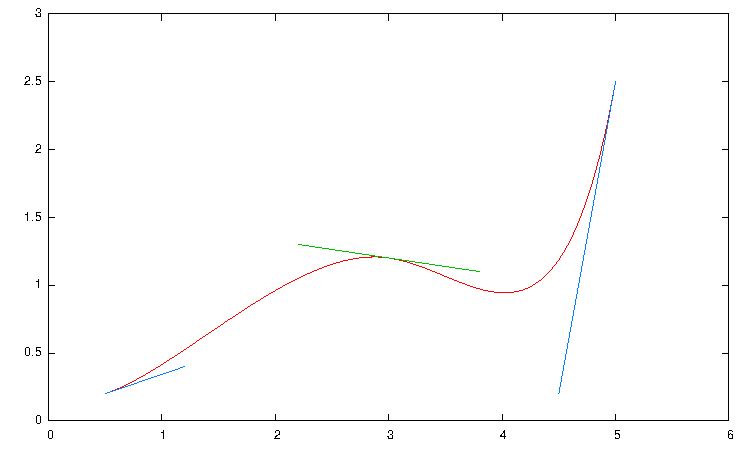
\includegraphics[scale=.7]{bezier2}
\caption{Two Bezier curves, joined together smoothly}
\label{fig:bezier2}
\end{figure}
\gnuplotsource{bezier2.gp}{The source for figure~\ref{fig:bezier2}}

\Level 1 {Drawing splines}

Even if we can evaluate a Bezier curve efficiently
(section~\ref{sec:bezier-calc}) in a given point, we can improve on
this considerably in the context of line drawing. Consider the problem
of drawing a cubic curve on the interval~$[0,1]$ by drawing
consecutive points~$Q(n\delta)$ for~$n=0,1,\ldots$.

We will discuss one line-drawing technique in the chapter on raster graphics.
A technique that is attractive for splines, and which is used in
\Metafont, is recursive subdivision. Here, a curve is subdivided until
a segment is a straight line within the pixel resolution, so that a
line drawing algorithm can be used. The test for a straight line can
be implemented efficiently through using the spline control points.

\endinput

\Level 1 {Bezier curves according to Knuth}

MT:43,44
\[ z(t) = 3t^2-2t^3+re^{i\theta}t(1-t)^2-se^{-i\phi}t^2(1-t) \]


\Level 1 {Other facts}

The blending function is always a polynomial one degree less than the
number of control points. Thus 3 control points results in a parabola,
4 control points a cubic curve etc.


Closed curves can be generated by making the last control point the
same as the first control point. First order continuity can be
achieved by ensuring the tangent between the first two points and the
last two points are the same.

As the number of control points increases it is necessary to have
higher order polynomials and possibly higher factorials. It is common
therefore to piece together small sections of BŽzier curves to form
a longer curve. This also helps control local conditions, normally
changing the position of one control point will affect the whole
curve. Of course since the curve starts and ends at the first and last
control point it is easy to physically match the sections. It is also
possible to match the first derivative since the tangent at the ends
is along the line between the two points at the end.  Second order
continuity is generally not possible.




Except for the redundant cases of 2 control points (straight line), it
is generally not possible to derive a BŽzier curve that is parallel
to another BŽzier curve.


A circle cannot be exactly represented with a BŽzier curve.

The degree of the curve is one less than the number of control points,
so it is a quadratic for 3 control points. It will always be symmetric
for a symmetric control point arrangement.






The curve always passes through the end points and is tangent to the
line between the last two and first two control points. This permits
ready piecing of multiple BŽzier curves together with first order
continuity.






The curve always lies within the convex hull of the control
points. Thus the curve is always "well behaved" and does not
oscillating erratically.
